\begin{ccRefClass} {Iso_cuboid_3<Kernel>}

\ccDefinition  An object $s$ of the data type \ccRefName\ is a
cuboid in the Euclidean space $\E^3$ with edges parallel to the $x$,
$y$ and $z$ axis of the coordinate system.
 
Although they are represented in a canonical form by only two
vertices, namely the lexicographically smallest and largest vertex
with respect to Cartesian $xyz$ coordinates, we provide
functions for ``accessing'' the other vertices as well.

Iso-oriented cuboids and bounding boxes are quite similar. The
difference however is that bounding boxes have always double coordinates, 
whereas the coordinate type of an iso-oriented cuboid is chosen by
the user.

\ccCreation
\ccCreationVariable{c}

\ccHidden \ccConstructor{Iso_cuboid_3();}
             {introduces an uninitialized variable \ccVar.}

\ccHidden \ccConstructor{Iso_cuboid_3(const Iso_cuboid_3<Kernel> &u);}
            {copy constructor.}

\ccConstructor{Iso_cuboid_3(const Point_3<Kernel> &p, 
                            const Point_3<Kernel> &q);}
            {introduces an iso-oriented cuboid \ccVar\ with diagonal
             opposite vertices $p$ and $q$. Note that the object is 
             brought in the canonical form.}

\ccConstructor{Iso_cuboid_3(const Point_3<Kernel> &p, 
                            const Point_3<Kernel> &q, int);}
            {introduces an iso-oriented cuboid \ccVar\ with diagonal
             opposite vertices $p$ and $q$.  The \ccc{int} argument value
             is only used to distinguish the two overloaded functions.
             \ccPrecond{$p.x()<=q.x()$, $p.y()<=q.y()$ and $p.z()<=q.z()$.}}

\ccConstructor{Iso_cuboid_3(const Point_3<Kernel> &left, 
                            const Point_3<Kernel> &right,
                            const Point_3<Kernel> &bottom,
                            const Point_3<Kernel> &top,
                            const Point_3<Kernel> &far,
                            const Point_3<Kernel> &close);}
            {introduces an iso-oriented cuboid \ccVar\ whose
             minimal $x$ coordinate is the one of \ccc{left}, the
             maximal $x$ coordinate is the one of \ccc{right}, the
             minimal $y$ coordinate is the one of \ccc{bottom}, the
             maximal $y$ coordinate is the one of \ccc{top}, the
             minimal $z$ coordinate is the one of \ccc{far}, the
             maximal $z$ coordinate is the one of \ccc{close}.}

\ccConstructor{Iso_cuboid_3(
                const Kernel::RT& min_hx, const Kernel::RT& min_hy, const Kernel::RT& min_hz,
                const Kernel::RT& max_hx, const Kernel::RT& max_hy, const Kernel::RT& max_hz,
                const Kernel::RT& hw = RT(1));}
            {introduces an iso-oriented cuboid \ccVar\ with diagonal
             opposite vertices 
             (\ccc{min_hx/hw}, \ccc{min_hy/hw}, \ccc{min_hz/hw}) and
             (\ccc{max_hx/hw}, \ccc{max_hy/hw}, \ccc{max_hz/hw}).  
             \ccPrecond \ccc{hw} $\neq$ 0.}


\ccOperations
\ccHidden \ccMethod{Iso_cuboid_3<Kernel> & operator=(const Iso_cuboid_3<Kernel> &q);}
        {Assignment.}

\ccMethod{bool operator==(const Iso_cuboid_3<Kernel> &c2) const;}
       {Test for equality: two iso-oriented cuboid are equal, iff their
        lower left and their upper right vertices are equal.}

\ccMethod{bool operator!=(const Iso_cuboid_3<Kernel> &c2) const;}
       {Test for inequality.}

\ccMethod{Point_3<Kernel> vertex(int i) const;}
       {returns the i'th vertex modulo 8  of \ccVar.
        starting with the lower left vertex.}

\ccMethod{Point_3<Kernel> operator[](int i) const;}
       {returns  \ccStyle{vertex(i)}, as indicated in the figure below:
       \lcTex{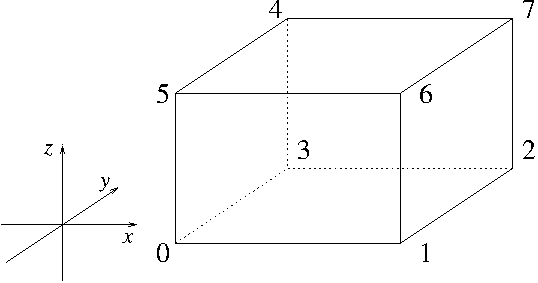
\includegraphics[width=6cm]{Kernel_23_ref/fig/IsoCuboid}}}

\begin{ccHtmlOnly}
<center>
<img border=0 src="fig/IsoCuboid.gif" align=center alt="vertex order of
  an iso-cuboid">
</center>
\end{ccHtmlOnly} 


\ccMethod{Point_3<Kernel> min() const;}
       {returns the smallest vertex of \ccVar\ (= \ccStyle{vertex(0)}).}


\ccMethod{Point_3<Kernel> max() const;}
       {returns the largest vertex of \ccVar\ (= \ccStyle{vertex(7)}).}
\ccMethod{ Kernel::FT  xmin() const;}{returns smallest \ccHtmlNoLinksFrom{Cartesian}
                              $x$-coordinate in \ccVar.}
\ccGlue
\ccMethod{ Kernel::FT  ymin() const;}{returns smallest \ccHtmlNoLinksFrom{Cartesian} 
                              $y$-coordinate in \ccVar.}
\ccGlue
\ccMethod{ Kernel::FT  zmin() const;}{returns smallest \ccHtmlNoLinksFrom{Cartesian} 
                              $z$-coordinate in \ccVar.}
\ccGlue
\ccMethod{ Kernel::FT  xmax() const;}{returns largest \ccHtmlNoLinksFrom{Cartesian} 
                              $x$-coordinate in \ccVar.}
\ccGlue
\ccMethod{ Kernel::FT  ymax() const;}{returns largest \ccHtmlNoLinksFrom{Cartesian} 
                              $y$-coordinate in \ccVar.}
\ccGlue
\ccMethod{ Kernel::FT  zmax() const;}{returns largest \ccHtmlNoLinksFrom{Cartesian} 
                              $z$-coordinate in \ccVar.}

\ccMethod{ Kernel::FT  min_coord(int i) const;}
         {returns $i$-th \ccHtmlNoLinksFrom{Cartesian} coordinate of
          the smallest vertex of \ccVar. 
%          (\ccc{min_coord(0) == xmin()}; \ccc{min_coord{2} == zmin()})
          \ccPrecond $0 \leq i \leq 2$.}

\ccMethod{ Kernel::FT  max_coord(int i) const;}
         {returns $i$-th \ccHtmlNoLinksFrom{Cartesian} coordinate of
          the largest vertex of \ccVar. 
%          (\ccc{max_coord(0) == xmax()}; \ccc{max_coord{2} == zmax()})
          \ccPrecond $0 \leq i \leq 2$.}

\ccPredicates

\ccMethod{bool is_degenerate() const;}
       {%the iso-oriented cuboid 
        \ccVar\ is degenerate, if all vertices
        are collinear.}

\ccMethod{Bounded_side bounded_side(const Point_3<Kernel> &p) const;}
       {returns either \ccStyle{ON_UNBOUNDED_SIDE},
        \ccStyle{ON_BOUNDED_SIDE}, or the constant
        \ccStyle{ON_BOUNDARY}, 
        depending on where point $p$ is.}

\ccMethod{bool has_on_boundary(const Point_3<Kernel> &p) const;}
       {}
\ccGlue
\ccMethod{bool has_on_bounded_side(const Point_3<Kernel> &p) const;}
       {}
\ccGlue
\ccMethod{bool has_on_unbounded_side(const Point_3<Kernel> &p) const;}
       {}

\ccHeading{Miscellaneous}

\ccMethod{Kernel::FT volume() const;}
       {returns the volume of \ccVar. }

\ccMethod{Bbox bbox() const;}
       {returns a bounding box containing \ccVar. }

\ccMethod{Iso_cuboid_3<Kernel>  transform(const Aff_transformation_3<Kernel> &t) const;}
       {returns the iso-oriented cuboid obtained by applying $t$ on 
        the smallest and the largest of \ccVar.
        \ccPrecond The angle at a rotation must be a multiple of $\pi/2$,
        otherwise the resulting cuboid does not have the same size.
        Note that rotating about an arbitrary angle can even result in
        a degenerate iso-oriented cuboid.}


\ccSeeAlso
\ccRefConceptPage{Kernel::IsoCuboid_3} \\

\end{ccRefClass} 
